\chapter{Schwarmrobotik und Evolutionäre Robotik}
\section{Schwärme  und deren Verhalten in der Natur}
\paragraph{Schwarmdefinition}
Der Begriff \textbf{Schwarm} bezeichnet einen Verband von fliegenden oder schwimmenden Lebewesen, der sich koordiniert bewegt.
Im Unterschied zu anderen Gruppen zeigt er ein sogenanntens \textbf{Schwarmverhalten}
\subsection{Computersimulation von Schwärmen - Algorithmus von Craig Reynolds}
Die einzelnen Individuen agieren in Abhängigkeit von der Position und der Geschwindigkeit der benachbarten Boids nach folgenden Regeln:
\paragraph{Separation} Bewege dich weg sobald dir andere zu nahe kommen
\paragraph{Alignment} Bewege dich in die gleiche Richtung wie deine Nachbarn
\paragraph{Cohesion} Bewege dich zum Mittelpunkt der benachbarten Vögel
\paragraph{Vorraussetzung}
Reynolds setzte vorraus, dass \textbf{alle} Vögel innerhalb eines fixen gegebenen Radius interagieren.
Die Nachbarschaft ist bei Reynolds charakterisiert durch einen Abstand vom Zentrum des Vogels und durch einen bestimmten Winkel ausgehend von der Flugrichtung.
Tiere außerhalb dieser Nachbarschaft werden ignoriert.
\section{Schwarmintelligenz}
Unter \textbf{Schwarmintelligenz} versteht man Systeme bestehend aus vielen primitiven, mobilen Agenten, die:
\begin{itemize}
	\item gemeinsam agieren
	\item miteinander kommunizieren können
	\item im Kollektiv ein komplexes Problem lösen
	\item ohne zentrale Steuerung sich selbst organisieren
\end{itemize}
\paragraph{Kollektive Intelligenz} Die Individuen agieren ziemlich beschränkt, die Gesellschaften dagegen sind ungemein leistungsfähig.
Geeignet zur \textbf{Lösung schwieriger Optimisierungsprobleme}
\section{Multi Robot Systems}
Einsatz von simplen Robotern, deren Handlungsmöglichkeiten und Wahrnehmungssysteme stark begrenzt sind.
\paragraph{Vorteile}
\begin{itemize}
	\item \textbf{robust}
	\item \textbf{skalierbar}
	\item \textbf{flexibel}
	\item \textbf{Kosten} statt eines euren einzelnen Roboters, der eventuell nicht so leicht oder schnell zu ersetzen ist, werden billige Komponenten eingesetzt.
	\item \textbf{Verlässlichkeit} wenn ein einzelner Roboter oder Softwareagent ausfällt übernehmen andere Roboter dessen Aufgabe und fügen sich neu ins Kollektiv
	\item \textbf{Flexibilität} viele kleine kooperierende Roboter können bei sinnvoller Zusammenarbeit Probleme bewältigen, die ein großer Roboter alleine eventuell nicht bewältigen kann.
\end{itemize}
\paragraph{Problem} Das Schwarmverhalten ist aufgrund des Einzelverhaltens nur schwer vorhersagbar.
\section{Ameisenalgorithmen}
\subsection{Optimaler Weg bei futtersbeschaffenden Ameisen}
\paragraph{Funktionsweise}
\begin{itemize}
	\item Eine Ameise verlässt den Bau, das nest (N) und sucht Futter auf einem \textbf{zufälligen Weg}
	\item Es gibt mehrere Zweige zur Futterquelle
	\item Weg wird mit \textbf{Pheromon}, einer chemischen Substanz markiert.
	\item Findet die Ameise Futter, schleppt sie das Futter auf dem gleichen oder einem anderen Weg zurück, der Weg wird dabei ev. ein weiteres Mal markiert.
	\item Weitere Ameisen, die zur Futtersuche starten, \textbf{orientieren sich} bei der Futtersuche \textbf{an den Pheromonspuren}
	\item Ameisen folgen \textbf{bevorzugt}, aber nicht immer den markierten Wegen
	\item Auf langen Wegen ist die Ameisendichte wegen der größeren Entfernung geringer, das Pheromon verdunstet schneller.
	\item Wenn ein Ausreißer einen kürzeren Weg findet und einige andere Ameisen beginnen diesem Weg zu folgen, wird die Ameisendichte auf dem längerenWeg immer geringer und der kürzere Weg setzt sich durch
\end{itemize}
\begin{figure}[H]
	\begin{center}
		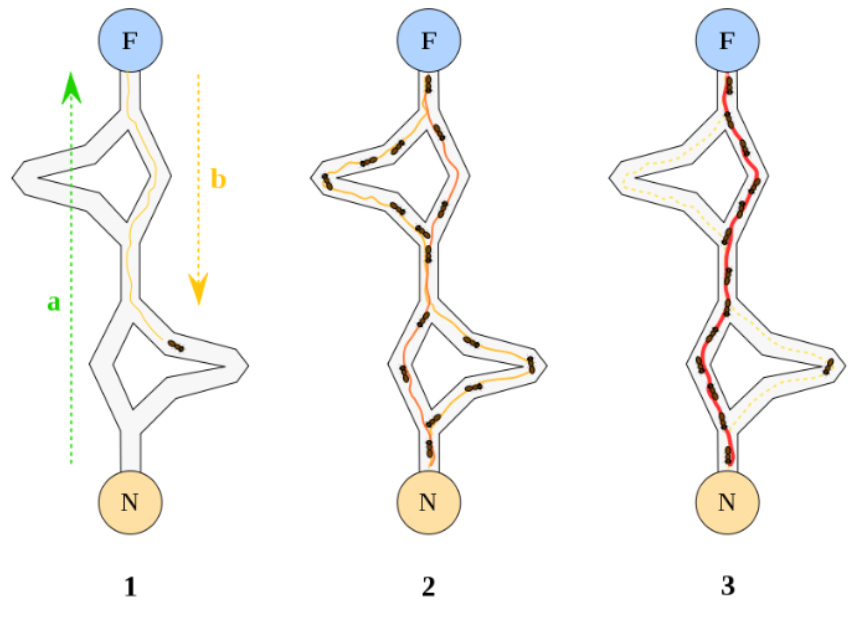
\includegraphics[scale=0.6]{Resources/PNG/AmeisenAlgorithmus.PNG}
		\caption{Darstellung des Ameisenalgorithmus Prinzips}
		\label{fig:PNG/AmeisenAlgorithmus.PNG}
	\end{center}
\end{figure}
\subsection{Ant Colony Optimization Algorithm}
\begin{itemize}
	\item \textbf{Ant Colony Optimization(ACO)} ist der Überbegriff für Ameisen-basierende Algorithmen
\end{itemize}
\paragraph{Kategorien}
\begin{itemize}
	\item \textbf{Tourenplanung (Routing)}: $\Rightarrow$ Travelling Salesman Problem
	\item \textbf{Zuordnung (Assignment)}: optimale Zuordnung von Personen oder Betriebsmitteln auf Stellen oder Aufgaben
	\item \textbf{Ablaufplanung (Scheduling)}: Verteilung von knappen Ressourcen auf Prozesse die zeitlich begrenzt sind
	\item \textbf{Teilmengen Problem (Subset)}: aus einer Menge von Objekten muss eine Teilmenge gefunden werden, damit eine vorgegebene Bedingung erfüllt und eine Zielfunktion optimiert wird. 
\end{itemize}
\paragraph{Eigenschaften}
\begin{itemize}
	\item optimaler Weg ist der \textbf{kürzeste Weg} zwischen zwei Punkten
	\item \textbf{globale Information}: Belegung mit künstlichen Pheromonen als zentrale Idee
	\item Wahrscheinlichkeits-gestützte, \textbf{lokale Entscheidungen} - Ameise erkennt unmittelbare Nachbarschaft
\end{itemize}
\paragraph{Funktionsweise}
\begin{enumerate}
	\item Ameisen laufen entlang des Graphen
	\item Eine Ameise erzeugt eine Lösung gemäß lokaler Information und Pheromon
	\item Update beinhaltet neu aufgetragene Pheromone und Verdunstung bereits vorhandener Pheromone
	\item Operationen, die globales Wissen vorraussetzen und damit nicht von einzelnen Ameisen bewerkstelligt werden können
\end{enumerate}
\begin{itemize}
	\item Diskretisierung der Zeit t: in einem Zeitschritt erzeugen alle Ameisen eine vollständige Lösung.
	\item Eine \textbf{Pheromon-Matrix} enthält die  Intensität der Pheromone $T_ij(t)$ enthält die Intensität der Pheromone auf einer Kante vom Knoten $i$ zum Knoten $j$ im Graphen
	\item Eine Matrix für lokale Informationen enthält die Sichtbarkeit der Stadt (d.h. die jeweils reziproke Distanz): $n_ij = \dfrac{1 }{d_ij}$
\end{itemize}
\subsection{Traveling Salesman Problem}
\begin{itemize}
	\item Vorhanden: \textbf{vollständiger gerichteter Graph} 
	\item Gesucht: \textbf{Rundtour durch alle Städte}
\end{itemize}
Ameisen laufen durch den Graphen, die Kolonie ermittelt den Optimalen Weg.
\begin{itemize}
	\item Es erweist sich als vorteilhaft, für jede Ameise eine andere zufällig gewählte Stadt als Ausgangspunkt für die Tour zu nehmen
\end{itemize}
\paragraph{Algorithmus - Schritte}
\begin{figure}[H]
	\begin{center}
		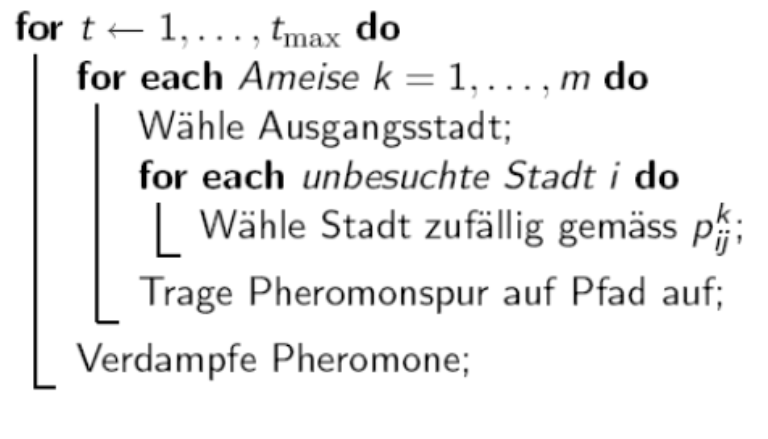
\includegraphics[scale=0.5]{Resources/PNG/ACO.PNG}
		\caption{Ameisenalgorithmus - Schritte}
		\label{fig:PNG/ACO.PNG}
	\end{center}
\end{figure}
\paragraph{Entscheidung für nächste Stadt}
\begin{itemize}
	\item Jede Ameise besitzt eine Liste mit gültiger Nachbarschaft $N$
	\item Die Entscheidung in einem Knoten bzgl. der nächsten Stadt fällt gemäß folgender Formel:
\end{itemize}
$p_{i j}^{k}=\left\{\begin{array}{ll}{\frac{\left[\tau_{i j}(t)\right]^{\alpha} \cdot\left[\eta_{i j}\right]^{\beta}}{\sum_{l \in J_{i}^{k}}\left[\tau_{i l}(t)\right]^{\alpha} \cdot\left[\eta_{i l}\right]^{\beta}}} & {\text { für } j \in J_{i}^{k}} \\ {0} & {\text { für } j \notin J_{i}^{k}}\end{array}\right.$
\begin{itemize}
	\item $\alpha$ und $\beta$ steuern das Verhältnis zwischen Anteil der Pheromone und lokaler Information
	\item für $\alpha$ hat man den klassischen Greedy Ansatz
\end{itemize}


